\documentclass[10pt]{article}
\usepackage{mathpaper}
\usepackage{tabularx}

\begin{document}
\showsecret
\papertitle{九年级上册期末质量检测一}
\centerline{\Large 答题卡}
\informationline
\textbf{\selectingintroduction}
\begin{table}[!htb]
    \centering
    \begin{tabularx}{\textwidth}{|*{11}{>{\centering\arraybackslash}X|}} \hline
        题号 & 1 & 2 & 3 & 4 & 5 & 6 & 7 & 8 & 9 & 10 \\ \hline
        选项 & \quad & \quad & \quad & \quad & \quad & \quad & \quad & \quad & \quad & \quad \\ \hline
    \end{tabularx}
\end{table}
\par \textbf{\complitingintroduction}
\begin{table}[!htb]
    \centering
    \renewcommand\arraystretch{1.5}
    \begin{tabularx}{\textwidth}{*{3}{>{\centering\arraybackslash}X}}
        11.\complitingline\complitingline\complitingline & 12.\complitingline\complitingline\complitingline & 13.\complitingline\complitingline\complitingline \\
        14.\complitingline\complitingline\complitingline & 15.\complitingline\complitingline\complitingline & 16.\complitingline\complitingline\complitingline  \\
    \end{tabularx}
\end{table}

\setcounter{taskcounter}{16}
\begin{questions}{\answeringintroduction}
    \question \addspace
    \question %18
    \begin{subquestions}
        \subquestion \qquad
        \begin{figure}[!htb]
            \raggedleft
                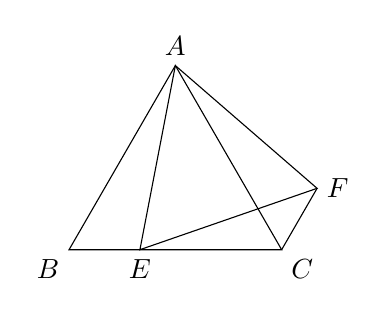
\begin{tikzpicture}[scale=0.45]
                    \coordinate[label=above:{$A$}] (A) at (3,5.19615);
                    \coordinate[label=below left:{$B$}] (B) at (0,0);
                    \coordinate[label=below right:{$C$}] (C) at (6,0);
                    \coordinate[label=below:{$E$}] (E) at (2,0);
                    \coordinate[label=right:{$F$}] (F) at (7,1.73205);
                    \draw (A) -- (B) -- (C) -- cycle;
                    \draw (A) -- (E) -- (F) -- cycle;
                    \draw (C) -- (F);
                \end{tikzpicture}
        \end{figure}
        \subquestion \addspace
    \end{subquestions}
    \question %19
    \begin{subquestions}
        \subquestion \complitingline\complitingline.
        \subquestion \newpage
    \end{subquestions}
    \question %20
    \begin{subquestions}
        \subquestion \addemptyline
        \subquestion \quad
        \begin{figure}[!htb]
            \raggedleft
                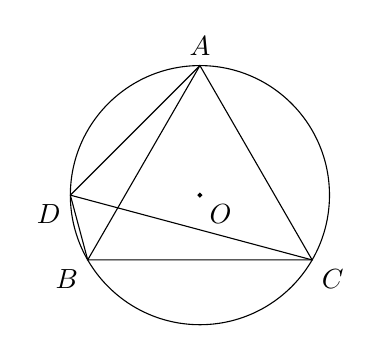
\begin{tikzpicture}[scale=0.475]
                    \coordinate[label=above:{$A$}] (A) at (3,5.19615);
                    \coordinate[label=below left:{$B$}] (B) at (0,0);
                    \coordinate[label=below right:{$C$}] (C) at (6,0);
                    \coordinate[label=below left:{$D$}] (D) at (-0.46410,1.73205);
                    \coordinate[label=below right:{$O$}] (O) at (3,1.73205);
                    \draw (A) -- (B) -- (C) -- cycle;
                    \filldraw (O) circle (0.05);
                    \draw (O) circle (3.46410);
                    \draw (A) -- (D);
                    \draw (B) -- (D);
                    \draw (C) -- (D);
                \end{tikzpicture}
        \end{figure}
    \end{subquestions}
    \question \qquad
    \begin{figure}[!htb]
        \raggedleft
            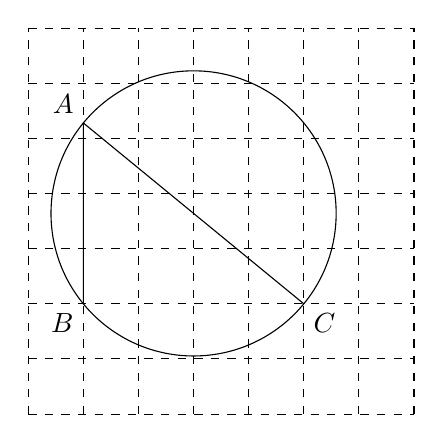
\begin{tikzpicture}[scale=0.7]
                \draw[step=1,dashed] (-1,-2) grid (6,5);
                \coordinate[label=below right:{$C$}] (C) at (4,0);
                \coordinate[label=above left:{$A$}] (A) at (0,3.28083);
                \coordinate[label=below left:{$B$}] (B) at (0,0);
                \draw (2,1.64042) circle (2.58669);
                \draw (B) -- (A) -- (C);
            \end{tikzpicture}
    \end{figure}
    \question %22
    \begin{subquestions}
        \subquestion \addemptyline
        \subquestion \addspace
        \subquestion \quad
        \begin{figure}[!htbp]
            \raggedleft
            \begin{tikzpicture}[scale=0.45,>=Stealth]
                \draw (-7,0) -- (10,0);
                \draw (3,5) -- (9,5);
                \coordinate (B) at (4,1);
                \coordinate (D) at (7.46410,3);
                \node[above right] at (8.14711,3) {$D$};
                \node[above right] at (4.25,0.75) {$B$};
                \coordinate[label=above:{$O$}] (O) at (4,5);
                \draw (B) -- (O);
                \draw[densely dashed] (O) -- (D);
                \draw (4,0.5) circle (0.5);
                \draw (-5,0.5) circle (0.5);
                \node[above right] at (-4.75,0.75) {$A$};
                \draw[densely dashed] (7.89711,2.75) circle (0.5);
                \draw[densely dashed] (0,0.5) circle (0.5);
                \draw[->] (-3.6,1.1) -- (-2.6,1.1) node[above left] {$v_1$};
                \draw[densely dashed] (2.3,2.75) -- (7.5,2.75);
                \node[left] at (2.5,1.375) {$h$};
                \draw[<->] (2.5,0.1) -- (2.5,2.74);
                \draw[densely dashed] (4,0.5) arc (270:330:4.5);
            \end{tikzpicture}
        \end{figure} \newpage
    \end{subquestions}
    \question %23
    \begin{subquestions}
        \subquestion \quad
        \begin{figure}[!htb]
            \raggedleft
            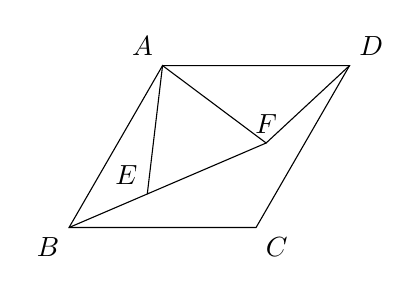
\begin{tikzpicture}[scale=0.475]
                \coordinate[label=above left:{$A$}] (A) at (2.5,4.33013);
                \coordinate[label=below left:{$B$}] (B) at (0,0);
                \coordinate[label=below right:{$C$}] (C) at (5,0);
                \coordinate[label=above right:{$D$}] (D) at (7.5,4.33013);
                \draw (A) -- (B) -- (C) -- (D) -- cycle;
                \coordinate[label=above left:{$E$}] (E) at (2.09151,0.89705);
                \coordinate[label=above:{$F$}] (F) at (5.26889,2.25983);
                \draw (A) -- (E) -- (F) -- cycle;
                \draw (B) -- (E);
                \draw (D) -- (F);
            \end{tikzpicture}
        \end{figure}
        \subquestion \quad
        \begin{figure}[!htb]
            \raggedleft
            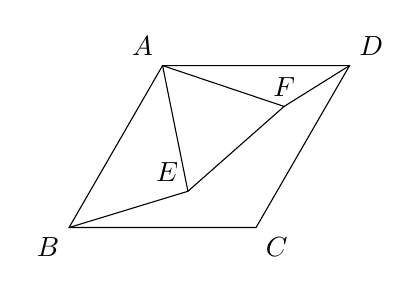
\begin{tikzpicture}[scale=0.475]
                \coordinate[label=above left:{$A$}] (A) at (2.5,4.33013);
                \coordinate[label=below left:{$B$}] (B) at (0,0);
                \coordinate[label=below right:{$C$}] (C) at (5,0);
                \coordinate[label=above right:{$D$}] (D) at (7.5,4.33013);
                \draw (A) -- (B) -- (C) -- (D) -- cycle;
                \coordinate[label=above left:{$E$}] (E) at (3.17839,0.96984);
                \coordinate[label=above:{$F$}] (F) at (5.74929,3.23749);
                \draw (A) -- (E) -- (F) -- cycle;
                \draw (B) -- (E);
                \draw (D) -- (F);
            \end{tikzpicture}
        \end{figure} \addspace \addspace
        \subquestion \addemptyline
    \end{subquestions}
    \question %24
    \begin{subquestions}
        \subquestion
        \begin{subsubquestions}
            \subsubquestion \complitingline\complitingline ;\complitingline\complitingline .\addemptyline
            \subsubquestion \complitingline\complitingline.
        \end{subsubquestions}
        \subquestion \quad
        \begin{figure}[!htb]
            \raggedleft
            \begin{tikzpicture}[>=Stealth,scale=0.5]
                \draw[->] (-4,0) -- (4,0) node[below] {$x$};
                \draw[->] (0,-1) -- (0,5) node[right] {$y$};
                \coordinate[label=below right:{$O$}] (O) at (0,0);
                \coordinate[label=right:{$F$}] (F) at (0,2);
                \draw (-4,5) parabola bend (0,1) (4,5);
                \coordinate[label=right:{$P$}] (P) at (-3,3.25);
                \draw (P) circle (3.25);
                \draw (O) -- (-4,4.3333);
            \end{tikzpicture}
        \end{figure} \newpage
        \subquestion \quad
        \begin{figure}[!htb]
            \raggedleft
            \begin{tikzpicture}[>=Stealth,scale=0.5]
                \draw[->] (-4,0) -- (4,0) node[below] {$x$};
                \draw[->] (0,-1) -- (0,5) node[right] {$y$};
                \coordinate[label=below right:{$O$}] (O) at (0,0);
                \coordinate[label=right:{$F$}] (F) at (0,2);
                \draw (-4,5) parabola bend (0,1) (4,5);
                \coordinate[label=below left:{$P$}] (P) at (-3,3.25);
                \coordinate[label=below right:{$Q$}] (Q) at (1.333333,1.444444);
                \coordinate[label=below:{$T$}] (T) at (-0.83333,0);
                \draw (P) -- (Q) -- (T) -- cycle;
                \draw (F) -- (T);
            \end{tikzpicture}
        \end{figure}
    \end{subquestions}
\end{questions}
\end{document}